\chapter{Mission: Breach Point}

\emph{\emph{Breach Point} is a RECON+ mission to secure an entry point
  into a quadrant of Dr.~Tokh's campus.}

\section{Play Area}
\vspace{-2\parskip}
\noindent\begin{stdminipage}{\linewidth-(2in+1.5em)}
\vspace{0pt}   
\noindent
Whichever player takes Deployment in the Initiative Roll chooses
either of the long edges of the play area as the Breach Point.

There is an Exclusion Zone~6'' along the the Breach Point edge extent.

The Deployment Zones are clipped triangles along the short edges
stretching from~3'' forward of that edge along the inner Exclusion
Zone boundary, to the point~12'' forward on the opposite edge of the
play area (this may also be measured by stretching a line from the
corner inside the Exclusion Zone to a point~12'' forward on the far
play area edge, with no models permitted to be deployed inside the
Exclusion Zone).

There are two scoring Sectors: The Target Sector, extending~6'' from
the Breach Point edge and~4'' on either side of the short centerline;
and the Approach Sector, extending~12'' from the Breach Point edge
and~9'' on either side of the short centerline but excluding the
Target Sector.

A Network Terminal is placed on the short center axis of the
table,~4'' from the long play area edge opposite the Breach Point
edge.
\end{stdminipage}
\hfill
\begin{minipage}[t]{2in}\centering
\vspace{4pt}   
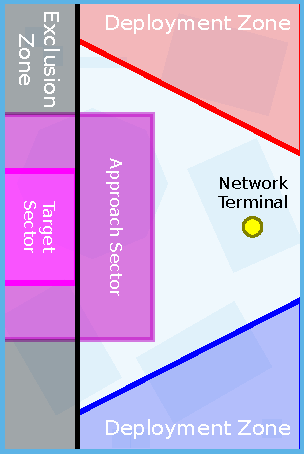
\includegraphics{maps/map-breachpoint}

\medskip\small%
\emph{(flip if opposite long edge chosen as the Breach Point)}
\end{minipage}

\section{Mission Rules}

Special Agents count as an additional 30 army points for purposes of
calculating domination.

\section{Scoring}

Players may score up to~10 objective points via the following
conditions at game end:
\begin{squishitemize}
\item 1pt for having a model with more than half its base inside the
  Approach Sector.
\item 2pts for dominating the Approach Sector.
\item 2pt for having a model with more than half its base inside the
  Target Sector.
\item 3pts for dominating the Target Sector.
\item 1pt if the opposing Special Agent is in a Null state or eliminated.
\item 1pt if more points of the opposing army list have been destroyed.
\end{squishitemize}

\vfill
\vbox to 0pt{}